%----------------------------------------------------------------------------------------
%	PACKAGES AND OTHER DOCUMENT CONFIGURATIONS
%----------------------------------------------------------------------------------------

\documentclass[
10pt, % Main document font size
a4paper, % Paper type, use 'letterpaper' for US Letter paper
oneside, % One page layout (no page indentation)
%twoside, % Two page layout (page indentation for binding and different headers)
headinclude,footinclude, % Extra spacing for the header and footer
BCOR5mm, % Binding correction
]{scrartcl}


%%%%%%%%%%%%%%%%%%%%%%%%%%%%%%%%%%%%%%%%%
% Arsclassica Article
% Structure Specification File
%
% This file has been downloaded from:
% http://www.LaTeXTemplates.com
%
% Original author:
% Lorenzo Pantieri (http://www.lorenzopantieri.net) with extensive modifications by:
% Vel (vel@latextemplates.com)
%
% License:
% CC BY-NC-SA 3.0 (http://creativecommons.org/licenses/by-nc-sa/3.0/)
%
%%%%%%%%%%%%%%%%%%%%%%%%%%%%%%%%%%%%%%%%%

%----------------------------------------------------------------------------------------
%	REQUIRED PACKAGES
%----------------------------------------------------------------------------------------

\usepackage[
nochapters, % Turn off chapters since this is an article        
beramono, % Use the Bera Mono font for monospaced text (\texttt)
eulermath,% Use the Euler font for mathematics
pdfspacing, % Makes use of pdftex’ letter spacing capabilities via the microtype package
dottedtoc % Dotted lines leading to the page numbers in the table of contents
]{classicthesis} % The layout is based on the Classic Thesis style

\usepackage{arsclassica} % Modifies the Classic Thesis package

\usepackage[T1]{fontenc} % Use 8-bit encoding that has 256 glyphs

\usepackage[utf8]{inputenc} % Required for including letters with accents

\usepackage{graphicx} % Required for including images
\graphicspath{{Figures/}} % Set the default folder for images

\usepackage{enumitem} % Required for manipulating the whitespace between and within lists

\usepackage{lipsum} % Used for inserting dummy 'Lorem ipsum' text into the template

\usepackage{subfig} % Required for creating figures with multiple parts (subfigures)

\usepackage{amsmath,amssymb,amsthm} % For including math equations, theorems, symbols, etc

\usepackage{varioref} % More descriptive referencing

\usepackage{amsmath}

\usepackage{tcolorbox}

\tcbuselibrary{theorems}

\newtcbtheorem[]{mydef}{Definition}%
{colback=white!5,colframe=black!35!black,fonttitle=\bfseries}{def}


%----------------------------------------------------------------------------------------
%	THEOREM STYLES
%---------------------------------------------------------------------------------------

\theoremstyle{definition} % Define theorem styles here based on the definition style (used for definitions and examples)
\newtheorem{definition}{Definition}

\theoremstyle{plain} % Define theorem styles here based on the plain style (used for theorems, lemmas, propositions)
\newtheorem{theorem}{Theorem}

\theoremstyle{remark} % Define theorem styles here based on the remark style (used for remarks and notes)

%----------------------------------------------------------------------------------------
%	HYPERLINKS
%---------------------------------------------------------------------------------------

\hypersetup{
%draft, % Uncomment to remove all links (useful for printing in black and white)
colorlinks=true, breaklinks=true, bookmarks=true,bookmarksnumbered,
urlcolor=webbrown, linkcolor=RoyalBlue, citecolor=webgreen, % Link colors
pdftitle={}, % PDF title
pdfauthor={\textcopyright}, % PDF Author
pdfsubject={}, % PDF Subject
pdfkeywords={}, % PDF Keywords
pdfcreator={pdfLaTeX}, % PDF Creator
pdfproducer={LaTeX with hyperref and ClassicThesis} % PDF producer
} % Include the structure.tex file which specified the document structure and layout

\usepackage{amsmath}

\hyphenation{Fortran hy-phen-ation} % Specify custom hyphenation points in words with dashes where you would like hyphenation to occur, or alternatively, don't put any dashes in a word to stop hyphenation altogether

%----------------------------------------------------------------------------------------
%	TITLE AND AUTHOR(S)
%----------------------------------------------------------------------------------------

\title{\normalfont\spacedallcaps{NUTRIENT-LIMITATION IN COMPLEX MEDIUM}} % The article title

\subtitle{(not a paper draft)} % Uncomment to display a subtitle

% \author{\spacedlowsmallcaps{John Smith* \& James Smith\textsuperscript{1}}} % The article author(s) - author affiliations need to be specified in the AUTHOR AFFILIATIONS block

\date{} % An optional date to appear under the author(s)

%----------------------------------------------------------------------------------------

\begin{document}

%----------------------------------------------------------------------------------------
%	HEADERS
%----------------------------------------------------------------------------------------

\renewcommand{\sectionmark}[1]{\markright{\spacedlowsmallcaps{#1}}} % The header for all pages (oneside) or for even pages (twoside)
%\renewcommand{\subsectionmark}[1]{\markright{\thesubsection~#1}} % Uncomment when using the twoside option - this modifies the header on odd pages
\lehead{\mbox{\llap{\small\thepage\kern1em\color{halfgray} \vline}\color{halfgray}\hspace{0.5em}\rightmark\hfil}} % The header style

\pagestyle{scrheadings} % Enable the headers specified in this block

\maketitle % Print the title/author/date block

\setcounter{tocdepth}{2} % Set the depth of the table of contents to show sections and subsections only

%----------------------------------------------------------------------------------------
%	MODELS
%----------------------------------------------------------------------------------------

\section{NUTRIENT LIMITATION}
\label{sec:cell_lep}

\begin{mydef}{Nutrient Limitation}{nut_lim}
We consider a network to be nutrient limited by metabolite $A$ if:
$$\delta |U_z| / \delta |U_A| > 0$$
for some range $U_A \in [0, C]$ (an intake regime).
Where $U_z$ is the biomass upper maximum feasible value and
$U_A$ is the maximum uptake value allowed for metabolite $A$.
\end{mydef}

\begin{mydef}{Essential nutrient}{ess_nut}
We consider a metabolite $E$ to be essential if:
$$\lim_{|U_E| \to 0} |U_z| = 0$$
and
$$\lim_{|U_E| \to +\infty} |U_z| > 0$$
\end{mydef}

Our aim is to discuss the main network configurations which might lead to condition \ref{def:nut_lim}.

\subsection{MODEL}

The aim is to explore the network reduction space so we can find configurations where the desired nutrient is limited.
Using an abstract network model, we can study the different mechanisms which lead to nutrient limitation.
The model is defined using total reactions, that is, $S \Rightarrow P$ does not necessarily means that it is a single reaction,
it represents all reactions, or pathways, that produce $P$ from $S$. The model has the follow general reactions:

\begin{itemize}[label=$$]
\item Exchange reactions
\begin{itemize}[label=$$]
\item $Ex\_A$: $(-1)~A \Leftarrow$
\item $Ex\_E$: $(-1)~E \Leftarrow$
\item $Ex\_S$: $(-1)~S \Leftarrow$
\end{itemize}
\item Biomass equation
\begin{itemize}[label=$$]
\item $z$: $(-1)~E + (-1)~P_1 + (-1)~P_2 \Rightarrow$
\end{itemize}
\item Internal reactions
\item : $(-1)~A \Rightarrow ~P_1$
\item : $(-1)~A \Rightarrow ~P_2$
\item : $(-1)~S \Rightarrow ~P_1$
\item : $(-1)~S \Rightarrow ~P_2$
\end{itemize}

The model has three nutrients $E$, $A$ and $S$: $E$ is an always essential, $A$ is the metabolite of interest and $S$
is another general metabolite, which compete with $A$ for being limiting.
Also, the model has internal general reactions
connecting the nutrients with the biomass components $P_1$, $P_2$.
That means, neither $A$ nor $S$ alone are essentials.


\begin{figure}[h]
\centering
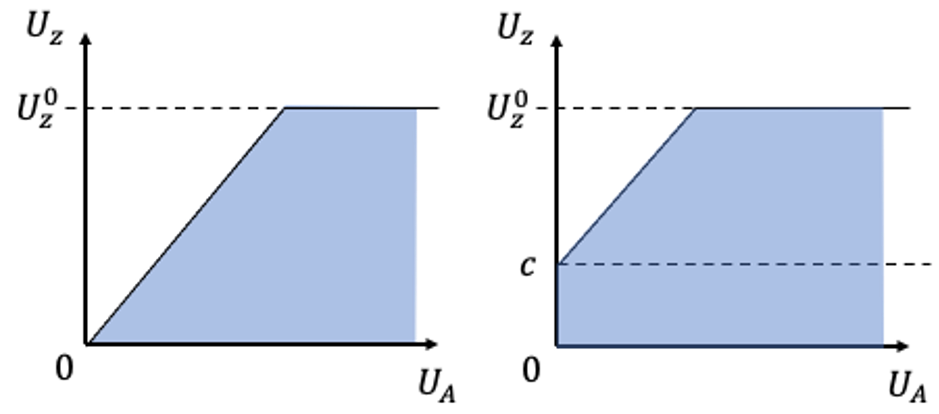
\includegraphics[width=0.8\columnwidth]{images/limiting_cases.png}
\caption[]{The two possible limiting cases.
$U_z$ is the upper limit for $z$ given all constraints other than $U_z^0$.
$U_A$ is the upper limit for the intake of $A$.
$c$ is the value of $z$ achievable without intaking any $A$.
Note that in a general network, the line of dependency could have changes on slope (due to changes in yield),
but the main feature of continuous regions of limitations (with non zero slope) remains general.
See main text for more analysis.
}
\label{fig:limiting_cases}
\end{figure}

Assuming that $z=0$ is inside the polytope (a vertex),
the convex nature of it allow us to conclude that there is only two possibilities for
$A$ to be limiting: i) $A$ to be essential (left panel Figure \ref{fig:limiting_cases}),
and ii) $A$ to be what I call $z > c$ limiting (right panel).

In case (i), there is at least one biomass component that can't be produced without $A$.
It would be the case if $S \Rightarrow ~P_1$ (or $S \Rightarrow ~P_2$) is knocked out, or
if the intake of $S$ is blocked.
Case (ii) is just a relaxed version of the first. The network is able to grow without $A$, but till a maximum $c$.
Above that threshold, $A$ is required and becomes a limiting factor.
In our model, setting $(S \Rightarrow ~P_1) < a$ produces such a situation, given that $z < U_z^0$ at $U_A = 0$.
The same is true if the intake of $S$ is restricted enough, $A$ can become limiting.
Note how in the last example, both nutrients $S$ and $A$ will be limiting.

As can be noted, even in this small model, there are several configurations which leads to nutrient limitation.
Is this degeneracy which complicates the contextualization of metabolic networks aimed to reproduce such phenotype.
One approach to learn about possible solutions is an exploration of the space of all limiting configurations.
Regarding possible exploration strategies, the two cases mentioned before have important differences.

All instances of case (i) rely inside the 'KO space'.
That is, all the configuration which has blocked reactions with respect to the original.
Without further constraints this space would be exponentially big with respect to the number of reactions.
But, we HOPE the network to be sensible enough so much of such space would be unfeasible.
The more reactions are blocked, the more probable it is for the network to yield zero biomass.
The good news is that at least, this space is well defined.

For the case (ii), the situation is more complicated.
We have continuous constraints $c$, which is harder to explore.
Plus, we might also have combinations of KO reactions and partial limitations which are compatible.
This space will be both hard to define and big.

\section{INTERESTING EXPERIMENTAL DATA}

We are trying to find experimental data which allows us to evaluate the importance of the nutrient limitation constraint over a metabolic model.
Ideally, we can manage to introduce into the model formulation the information contained in the phenotype of nutrient limitation, and with good luck,
this extra information might explain an improvement in the model performance.
Conversely, we can evaluate the risk of not taking into account such information.
That is, we shouldn't use models which fail to reproduce the experimental pattern of nutrient limitation, which is not uncommon practice in literature.
In general, for complex medium and/or mammalian cell cultures I haven't found good/clear/appropriate/interesting data in the literature.
Here are the main ones.

\subsection{CANCER AND GLYCINE}

At \cite{jainMetaboliteProfilingIdentifies2012} they evaluate the patterns of consumption/production of metabolites for a large set of cell lines
derived from cancer tissues.
A clear result is that for a subset of such lines glycine is strongly correlated with growth (see Figure \ref{fig:gly_cancer_corr}, left panel).

% Que Mulet se lea el paper y preguntarle dudas

\begin{figure}[h]
\centering
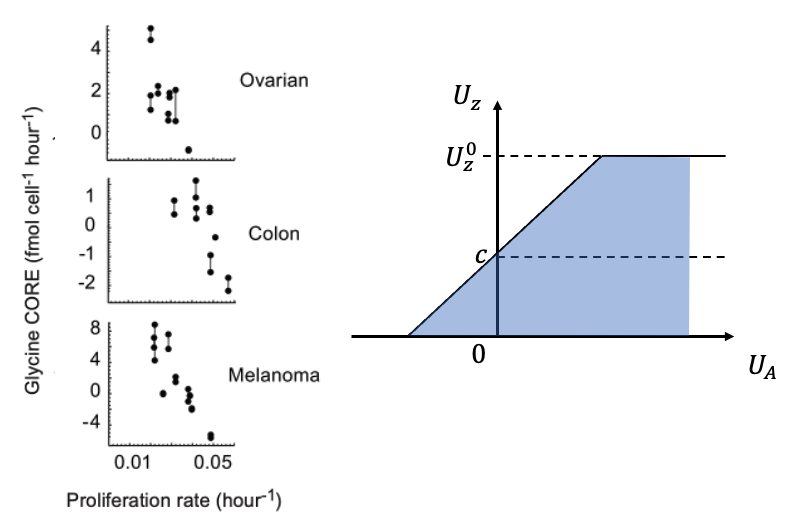
\includegraphics[width=0.8\columnwidth]{images/gly_cancer_corr.png}
\caption[]{
Left panel: Correlation between glycine exchange flux (y axis) and growth rate (x axis) for
cell lines extracted from three types of cancers. Reproduced without authorization from \cite{jainMetaboliteProfilingIdentifies2012}.
Right Panel: If you flip the axis and the convention for intakes/production, you realize that the trend is
compatible with a $z - c$ limitation (same as right panel on Figure \ref{fig:limiting_cases}), but this time the dependency is extended
also toward negative exchanges (production).
See main text for further analysis.
}
\label{fig:gly_cancer_corr}
\end{figure}

Quick analysis of this trend shows that glycine is not an essential metabolite, it is instead "$z > c$ limiting".
Actually, it is even more complicated that our initial definition of "nutrient limitation" because the trend is traceable till the production regime
(see Figure \ref{fig:gly_cancer_corr}, right panel).
That is, for $z < c$, glycine is still correlated with growth in the same way but it became a waste not a nutrient.
The authors also point out that this subset of lines with good correlations between gly and the proliferation rate are the ones growing
faster.

So, what can we do with this? The honest answer is "I don't know"! But let's talk about it.
This is still the best paper describing some kind of relationship between complex medium cultures growth rate and an external metabolite exchange.
Actually, the paper is very complete, it includes also transcriptomic screenings and an culture-supported hypothesis about why
glycine is important for fast growing cells.

From our point of view, we might want to see if including "somehow" into the model formulation just the nutrient limitation phenotype, we can
reproduce or get closer to, for instance, the same explanation for why glycine is important.
Or reproduce the general transcriptomic pattern.
Other approach could be to attempt to compute how likely from a naive point of view is the experimental configuration.
We can find, for instance, that because of an entropic effect, the experimental phenotype is backed by a dominant number of configurations.

What are the problems?
In previous attempts, we were trying to introduce/evalua-te the phenotype constraint by exploring the
ensemble of all nutrient-limited networks inside the KO feasible space.
That is, we were targeting a Figure \ref{fig:limiting_cases} left panel case.
This is the easier one because it only depends on the topology of the network (no free parameters).
But, even in this case, success was in jeopardy because the KO space is exponentially big and we are dearing to work
with the biggest available network of all, Human1.
On the other hand, the case at \cite{jainMetaboliteProfilingIdentifies2012} is obviously a $z > c$ limiting case.
Now we have a free parameter, the bottleneck constraint (the cause and value of $c$).
We need to introduce extra information, for instance, an intake/production set of constraints (which aren't reported in the paper).
Then, the results being sensible to its availability and accuracy.
This extra degeneracy means that this space is even bigger than just the KO space.
We now need to explore limiting (not blocking) the reactions of the network.

Ideas to think about:
i) In the experimental data we have the slope of the relationship between glycine and growth, not only the trend.
I suspect that this is a polytope edge. Yes, something is being optimized that is laid on this edge.
This slope is the shadow price of the glycine.
It will depend on the combination of the yields of the active elementary modes.
Again, for a case (i) this only depends on the topology, but for a case (ii), this is harder to explore,
because it depends on how you restrict the network.
ii) The fact that the correlation goes till the production part of the glycine exchange tells us that the
steady state assumption we make in the formulation of $Av = 0$ is accurate.

\subsection{RATH AND THE CHEMOSTAT}

Well, we have exchange fluxes from a set of cultures that the author \cite{rathCharacterisationCellGrowth2017} is reporting are glucose limited (see Figure \ref{fig:rath_time_serie}).
We can explore if marginalizing on the subnetworks which are glucose-limited we improve the reproduction of
such data compare with a random subnetwork.
We can explore just the KO space because it is easy.
The bad news is that reproducing fluxes is harder than just finding general KO patterns (transcriptomic data) based on topology.
Also, it is not a lot of data.

\begin{figure}[h]
\centering
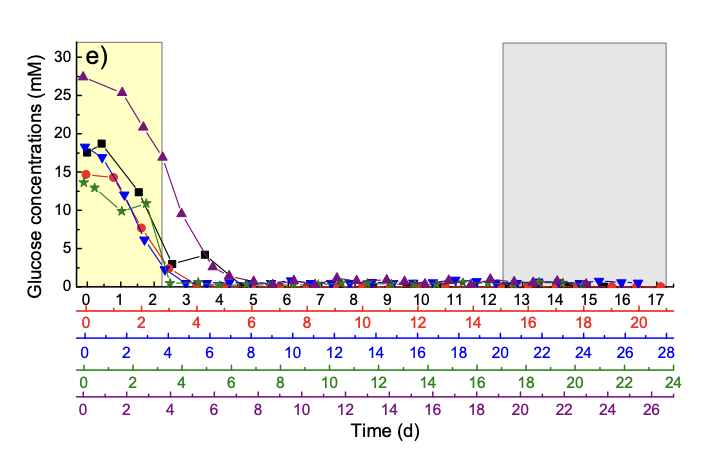
\includegraphics[width=0.8\columnwidth]{images/rath_time_serie.png}
\caption[]{
The time series of remaining glucose for 5 parallel continuous cultivations.
Reproduced without request from \cite{rathCharacterisationCellGrowth2017}
}
\label{fig:rath_time_serie}
\end{figure}

\section{SUMMARY}

Computations are probably unfeasible, questions aren't clear, data non available or noisy, rewards not very promising.
Unfortunately, just like 6 months ago.


% For us, this is important because that saids something about $c$ itself (that is "large") 


% Actuatlly, the authors did growth the cells with and without glycine for comparison (see Figure \ref{fig:gly_cancer_ko}). 
% Glycine became more and more "essental" as the cells displayed a larger proliferation rate.

% \begin{figure}[h]
%    \centering
%    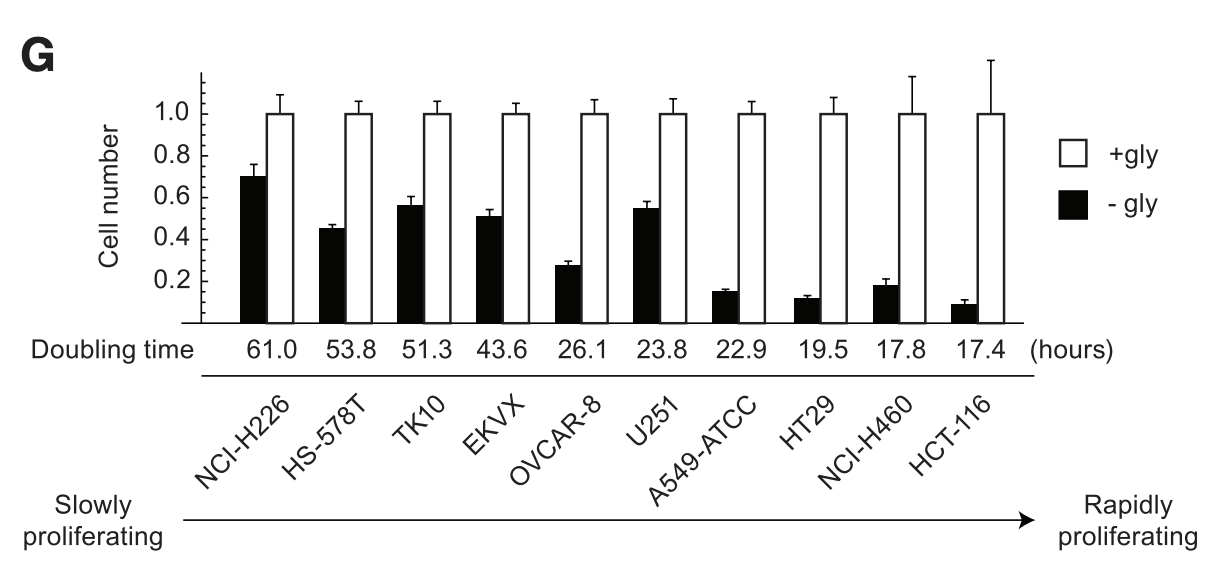
\includegraphics[width=0.8\columnwidth]{images/gly_cancer_ko.png}
%    \caption[]{
%       Reproduced without authorization from \cite{jainMetaboliteProfilingIdentifies2012}.
%    }
%    \label{fig:gly_cancer_ko}
% \end{figure}

% Whenever you find a linear dependency between fluxes, you are in an edge of the polytope?.






% First, let define the set of exchage reactions (the prefix $Ex\_$ denotes exchange), which input matter into the model. 
% \begin{itemize}[label=$$]
%    \item Exchange reactions
%    \begin{itemize}[label=$$]
%       \item $Ex\_A$:   $(-1)~A \Leftarrow$
%       \item $Ex\_E$: $(-1)~E \Leftarrow$
%       \item $Ex\_S$: $(-1)~S \Leftarrow$
%    \end{itemize}
% \end{itemize}

% Where: 
% Metabolite $E$ is an always essential metabolite.
% Metabolite $S$ is a non necesarilly essential metabolite.
% And $A$ is just a particular metabolite which is the focus of the analisis.

% Second, the biomass reaction is the sink of matter from the model.
% \begin{itemize}[label=$$]
%    \item Biomass equation
%    \begin{itemize}[label=$$]
%       \item $z$: $ (-1)E + (-1)P_1 + (-1)P_2 \Rightarrow$
%    \end{itemize}
% \end{itemize}


% Where: Metabolites $P_{*}$ are internal metabolites. 

% Finally, the internal reactions are the source of degeneracy of the system. 
% They introduce an exponentialy growing combinations of routes for matter to flow from the inputs (exchanges) to the sink (biomass).

% \begin{itemize}[label=$$]
%    \item Internal reactions

%    \begin{itemize}[label=$$]
%       \item $(-1)S \Rightarrow P_1$
%       \item $(-1)S \Rightarrow P_2$
%       \item $(-1)A \Rightarrow P_1$
%       \item $(-1)A \Rightarrow P_2$
%    \end{itemize}
% \end{itemize}

% Here we are considering each reaction as a total reaction (eg. $(-1)S \Rightarrow N P_1$ means that exist an open route from $S$ to $P_1$).

% Note that in the current configuration, assumming all exchanges are unbounded, the metabolite $A$ is neither limiting no essenctial.
% That is, the components of the biomass can be acquired from $S$.
% This situation can change if we do the follow transformations on the network:
% \begin{itemize}[label=$$]
   
%    \item i) Make $A$ essential: knocking the connections of $S$ to at least one component of $z$ which, at the same time, is reachable from $A$. For instance:
%    \begin{itemize}[label=$$]
%       \item Blocking $(-1)S \Rightarrow P_1$ will make $A$ the only source of $P_1$
%    \end{itemize}

%    \item ii) Create a bottleneck: If we limit (not block) the connection from $S$ to components of $z$, there will be always a regime of $z$ for which
%    $A$ is limiting. The case (i) is just an extreme of this one (where the regime of $z$ is all reals).
%    For instance: 
%    \begin{itemize}[label=$$]
%       \item If we limit $(-1)S \Rightarrow P_1$ so not all $P_1$ required for $z > C$ can be produced from $S$, 
%       $(-1)A \Rightarrow P_1$ will must the gap, and so, above this threshold, $z$ will depend on $Ex\_A$.
%    \end{itemize}
   
%    \item iii) Reduce the yield of $A$ under a defined medium: Here, reactions are blocked so the total ones (eg. $(-1)A \Rightarrow P_1$) reduces it yeild 
%    (eg. number of $P_1$ per $A$ produced, stoichiometric coefficients aren't shown). This can lead to the requirements of $z$ being to higt for 
%    the amount of $A$ and $S$ available in the deffined medium. This is different of the case (ii) because now we are not limiting the network capacity of 
%    consuming a nutrient, we are making it so ineficient that a previously suffitient resource become limiting.
   
%    \item iv) A combination of the previous

% \end{itemize}


% An important difference between the alternatives are the combinational space they produces (we will ignore (iv)). 
% The alternatives (i and ii) can be realized by exploring up to $2^{no. reactions}$ combinations.
% One per each KO/reduction pattern over the network. 

% \subsection{REDUCE THE COMBINATIONAL SPACE}




% \subsection{GENERAL MODEL}

% First, let define the set of exchage reactions (the prefix $Ex\_$ denotes exchange), which input matter into the model. 
% \begin{itemize}
%    \item Exchange reactions
%    \begin{itemize}
%       \item $Ex\_A$:   $(-1)~A \Leftarrow$
%       \item $Ex\_E_e$: $(-1)~E_e \Leftarrow$
%       \item $Ex\_S_s$: $(-1)~S_s \Leftarrow$
%    \end{itemize}
% \end{itemize}

% Where: 
% The set of metabolites $E_e$, $e \in [1,M_E]$, are the essential metabolites.
% The set of metabolites $S_s$, $s \in [1,M_S]$, are the non-essential metabolites.
% And $A$ is just a particular metabolite which is the target of the analisis.

% Second, the biomass reaction is the sink of matter from the model.

% \begin{itemize}
%    \item Biomass

%    \begin{itemize}
%       \item $z$:   $ \sum^{M_E} S_{ze} E_e + \sum^{M_S} S_{zs} E_s + S_{zA} A\Rightarrow$
%    \end{itemize}
% \end{itemize}

% The stoichiometric coefficients ($c_{*}$) control whom ultimatly is a biomass component. 

% Finally, the internal reactions are the source of degeneracy of the system. 
% They introduce an exponentialy growing combinations of routes for matter to flow from the inputs (exchanges) to the sink (biomass).
% We aim at 

% \begin{itemize}
%    \item Internal reactions

%    \begin{itemize}
%       \item $r_j$: $ \sum S_{ej} E_e \Rightarrow$
%    \end{itemize}
% \end{itemize}


































%----------------------------------------------------------------------------------------
%	BIBLIOGRAPHY
%----------------------------------------------------------------------------------------

\renewcommand{\refname}{\spacedlowsmallcaps{References}} % For modifying the bibliography heading

\bibliographystyle{unsrt}

\bibliography{report.bib} % The file containing the bibliography

%----------------------------------------------------------------------------------------

\end{document}